% This LaTeX was auto-generated from MATLAB code.
% To make changes, update the MATLAB code and export to LaTeX again.

\documentclass{article}

\usepackage[utf8]{inputenc}
\usepackage[T1]{fontenc}
\usepackage{lmodern}
\usepackage{graphicx}
\usepackage{color}
\usepackage{hyperref}
\usepackage{amsmath}
\usepackage{amsfonts}
\usepackage{epstopdf}
\usepackage[table]{xcolor}
\usepackage{matlab}

\sloppy
\epstopdfsetup{outdir=./}
\graphicspath{ {./bayesian_learning_images/} }

\begin{document}

\matlabtitle{Bayesian Learning}

\begin{par}
\begin{flushleft}
We are going to obtain data from a distribution $\mathcal{N}(5,2)$.
\end{flushleft}
\end{par}

\begin{matlabcode}
mu_true = 5;
sigma = 2;

num_samples = 10;

rng('default') % For reproducibility
data = mu_true + sigma_true * randn(num_samples, 1);

% Set up the x-axis for plotting
x = linspace(-5, 10, 1000);

% Plot the true distribution
figure;
hold on;
plot(x, normpdf(x, mu_true, sigma_true), 'LineWidth', 2);
title('Bayesian Learning');
xlabel('x');
ylabel('Probability Density');
xlim([-5, 10]);
legend('N(5, 2)');
\end{matlabcode}

\begin{par}
\begin{flushleft}
Our prior is going to be a standard normal $\mu \sim \mathcal{N}(0,1)$ and we are going to assume that $\sigma$ is well approximated by the sample variance.
\end{flushleft}
\end{par}

\begin{matlabcode}
mu_prior = 0;
sigma_prior = 1;
\end{matlabcode}

\begin{par}
\begin{flushleft}
Now, we are going to update our beliefs with the obtained datapoints, and the formulas for updating are:
\end{flushleft}
\end{par}

\begin{par}
$$\mu_n =\frac{\sigma_0^2 \sum x_i +\sigma^2 \mu_0 }{\sigma^2 +n\sigma_0^2 }$$ 
\end{par}

\begin{par}
\begin{flushleft}
and
\end{flushleft}
\end{par}

\begin{par}
\begin{flushleft}
$\sigma_n =\frac{\sigma^2 \sigma_0^2 }{\sigma^2 +n\sigma_0^2 }$.
\end{flushleft}
\end{par}

\begin{matlabcode}
mu_posterior = (sigma_prior^2*(sum(data))+var(data)*mu_prior)/(var(data)+num_samples*sigma_prior^2)
\end{matlabcode}
\begin{matlaboutput}
mu_posterior = 2.7734
\end{matlaboutput}
\begin{matlabcode}
sigma_posterior = (var(data)*sigma_prior^2)/(var(data)+num_samples*sigma_prior^2)
\end{matlabcode}
\begin{matlaboutput}
sigma_posterior = 0.5561
\end{matlaboutput}
\begin{matlabcode}

plot(x, normpdf(x, mu_posterior, sqrt(var(data))), 'LineWidth', 2);
xlabel('x');
ylabel('Probability Density');

sigma_prior = sigma_posterior;
mu_prior = mu_posterior;

data = mu_true + sigma_true * randn(num_samples, 1);

mu_posterior = (sigma_prior^2*(sum(data))+var(data)*mu_prior)/(var(data)+num_samples*sigma_prior^2)
\end{matlabcode}
\begin{matlaboutput}
mu_posterior = 4.0179
\end{matlaboutput}
\begin{matlabcode}
sigma_posterior = (var(data)*sigma_prior^2)/(var(data)+num_samples*sigma_prior^2)
\end{matlabcode}
\begin{matlaboutput}
sigma_posterior = 0.2034
\end{matlaboutput}
\begin{matlabcode}

plot(x, normpdf(x, mu_posterior, sqrt(var(data))), 'LineWidth', 2);
xlabel('x');
ylabel('Probability Density');

sigma_prior = sigma_posterior;
mu_prior = mu_posterior;

num_samples = 500;

data = mu_true + sigma_true * randn(num_samples, 1);

mu_posterior = (sigma_prior^2*(sum(data))+var(data)*mu_prior)/(var(data)+num_samples*sigma_prior^2)
\end{matlabcode}
\begin{matlaboutput}
mu_posterior = 4.7770
\end{matlaboutput}
\begin{matlabcode}
sigma_posterior = (var(data)*sigma_prior^2)/(var(data)+num_samples*sigma_prior^2)
\end{matlabcode}
\begin{matlaboutput}
sigma_posterior = 0.0064
\end{matlaboutput}
\begin{matlabcode}

plot(x, normpdf(x, mu_posterior, sqrt(var(data))), 'LineWidth', 2);
xlabel('x');
ylabel('Probability Density');
leg = legend('True distribution', 'Learned distribution', 'New learned distribution', 'New new');
leg.Location = "northwest"
\end{matlabcode}
\begin{center}
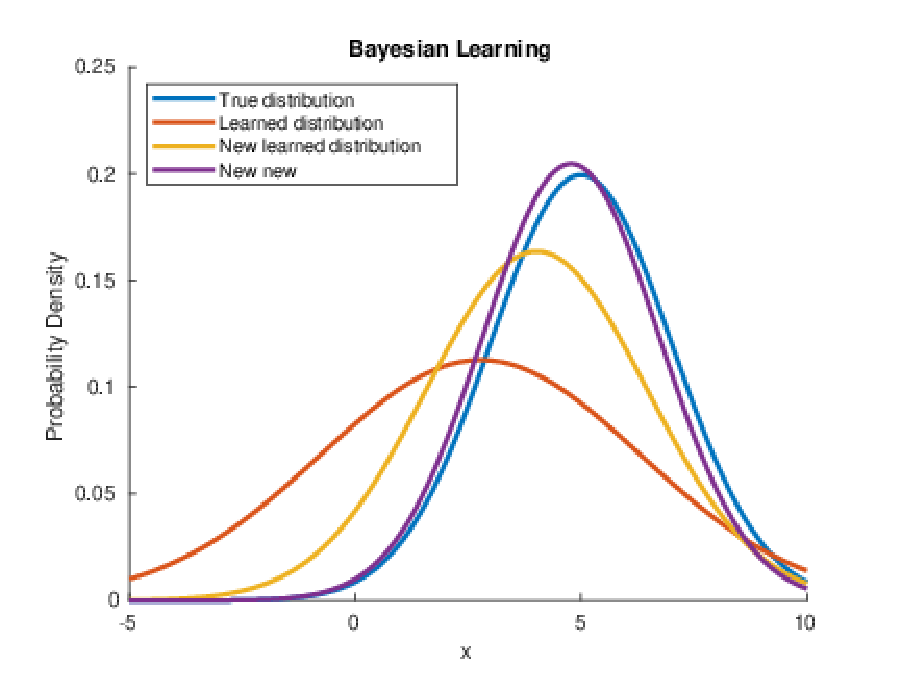
\includegraphics[width=\maxwidth{56.69844455594581em}]{figure_0.eps}
\end{center}
\begin{matlaboutput}
leg = 
  Legend (True distribution, Learned distribution, New learned distribution, New new) with properties:

         String: {'True distribution'  'Learned distribution'  'New learned distribution'  'New new'}
       Location: 'northwest'
    Orientation: 'vertical'
       FontSize: 9
       Position: [0.1483 0.7446 0.3565 0.1545]
          Units: 'normalized'

  Show all properties

\end{matlaboutput}

\end{document}
